\documentclass[aspectratio=169,11pt]{beamer}

\usetheme{Madrid}
\usecolortheme{default}
\setbeamertemplate{navigation symbols}{}
\setbeamertemplate{footline}[frame number]

\usepackage{amsmath,amssymb}
\usepackage{graphicx}
\usepackage{tikz}
\usetikzlibrary{positioning,calc}
\usetikzlibrary{arrows.meta,decorations.pathmorphing}

\definecolor{RamRed}{RGB}{190,40,45}
\definecolor{RamBlue}{RGB}{30,90,180}
\definecolor{SoftGray}{RGB}{245,245,245}
\definecolor{DarkGray}{RGB}{70,70,70}
\definecolor{MapGreen}{RGB}{48,150,95}
\definecolor{MapGold}{RGB}{235,180,45}

\setbeamercolor{title}{fg=DarkGray}
\setbeamercolor{frametitle}{fg=white,bg=RamBlue}
\setbeamercolor{structure}{fg=RamBlue}

\tikzset{
  v/.style={circle,draw=black,fill=white,inner sep=1.8pt},
  edge/.style={draw=RamBlue,line width=1.25pt},
  topic/.style={draw=black!30,fill=SoftGray,rounded corners=5pt,inner sep=7pt,
    text width=5.8cm,minimum height=1.65cm,align=left},
}


\usepackage{booktabs}
\tikzset{dot/.style={circle,fill=black,inner sep=2pt}, lab/.style={circle,draw=black,fill=white,inner sep=2pt,minimum size=6mm,font=\small},selected/.style={draw=RamRed,line width=2pt}}

\newcommand{\Def}[2]{\begin{block}{#1}#2\end{block}}
\newcommand{\Thm}[2]{\begin{block}{#1}#2\end{block}}
\renewcommand{\Proof}[1]{\begin{block}{Proof}\normalsize #1\end{block}}
\newcommand{\Question}[1]{\begin{block}{Question}#1\end{block}}
\renewcommand{\Example}[1]{\begin{block}{Example}#1\end{block}}
\newcommand{\fall}[2]{#1^{\underline{#2}}}
\newcommand{\rise}[2]{#1^{\overline{#2}}}
\newcommand{\stir}[2]{\left\{\begin{matrix}#1\\#2\end{matrix}\right\}}
\newcommand{\cyc}[2]{\left[\begin{matrix}#1\\#2\end{matrix}\right]}
\newcommand{\eul}[2]{\left\langle\begin{matrix}#1\\#2\end{matrix}\right\rangle}
\newcommand{\coef}[2]{[#1^{#2}]}
\newcommand{\gap}{\par\medskip}

\title{The Pigeonhole Principle}
\author{Jeremy Quastel}\date{}\begin{document}
\begin{frame}[plain]\begin{center}{\Huge\bfseries The Pigeonhole Principle}\par\vspace{.25cm}{\Large Section 2.4}\par\vspace{.15cm}{\large Harris--Hirst--Mossinghoff, \emph{Combinatorics and Graph Theory}}\par\vspace{.1cm}\resizebox{!}{2.7cm}{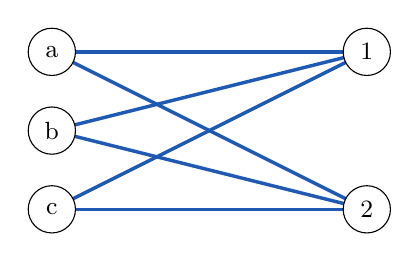
\begin{tikzpicture}[scale=1]
\coordinate (va) at (-2.000,1.000);
\coordinate (vb) at (-2.000,0.000);
\coordinate (vc) at (-2.000,-1.000);
\coordinate (v1) at (2.000,1.000);
\coordinate (v2) at (2.000,-1.000);
\draw[edge] (va)--(v1);
\draw[edge] (va)--(v2);
\draw[edge] (vb)--(v1);
\draw[edge] (vb)--(v2);
\draw[edge] (vc)--(v1);
\draw[edge] (vc)--(v2);
\node[lab] at (va) {a};
\node[lab] at (vb) {b};
\node[lab] at (vc) {c};
\node[lab] at (v1) {1};
\node[lab] at (v2) {2};
\end{tikzpicture}}\par\vspace{.25cm}Jeremy Quastel\end{center}\end{frame}
\begin{frame}[plain]\large \begin{center}{\Huge\bfseries Today\textquotesingle s lecture}\par\vspace{.5cm}\end{center}\begin{columns}[c,onlytextwidth]\begin{column}{.48\textwidth}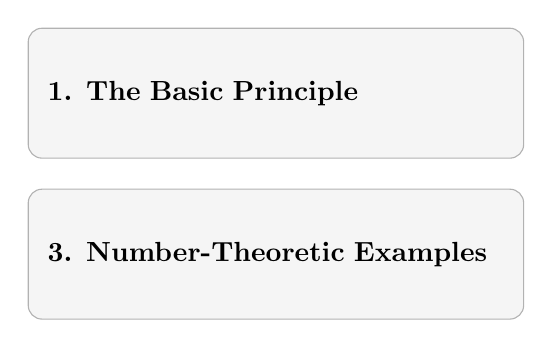
\begin{tikzpicture}\node[topic](a){\textbf{1. The Basic Principle}};\node[topic,below=.38cm of a]{\textbf{3. Number-Theoretic Examples}};\end{tikzpicture}\end{column}\begin{column}{.48\textwidth}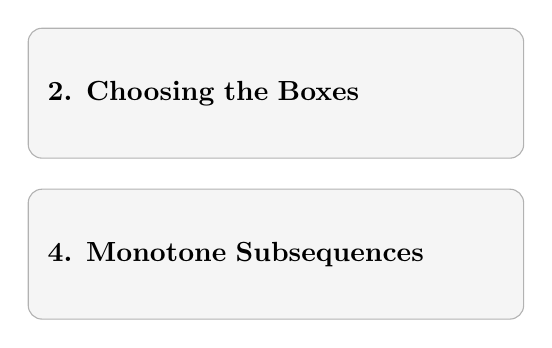
\begin{tikzpicture}\node[topic](a){\textbf{2. Choosing the Boxes}};\node[topic,below=.38cm of a]{\textbf{4. Monotone Subsequences}};\end{tikzpicture}\end{column}\end{columns}\end{frame}
\begin{frame}{An existence principle}
\large
\Question{If $13$ people are in a room, must two have birthdays in the same month?}
\gap There are $13$ people but only $12$ months. At least one month receives two people.
\gap We can force a coincidence without knowing which month it occurs in.
\end{frame}
\begin{frame}{The pigeonhole principle}
\large
\Thm{Pigeonhole principle}{If more than $n$ objects are placed in $n$ boxes, then some box contains at least two objects.}
\Proof{If every box contained at most one object, the total number of objects would be at most $n$, a contradiction.}
\end{frame}
\begin{frame}{The generalized principle}
\large
\Thm{Generalized pigeonhole principle}{If $N$ objects are placed in $k\geq1$ boxes, some box contains at least
\[\left\lceil\frac Nk\right\rceil\]
objects.}
\gap Equivalently, $k(r-1)+1$ objects force a box with at least $r$ objects.
\end{frame}
\begin{frame}{Proof of the generalized principle}
\large
\Proof{Suppose every box has at most $\lceil N/k\rceil-1$ objects. Since $\lceil N/k\rceil-1<N/k$, the total is less than
\[k\cdot\frac Nk=N,\]
a contradiction.}
\end{frame}
\begin{frame}{Choosing the boxes}
\large
\Def{A useful strategy}{Identify the desired coincidence, assign each object a label, and use the possible labels as boxes.}
\gap The hard part is usually finding the right labels.
\gap Remainders, degrees, parity patterns, and lengths of subsequences will all serve as boxes.
\end{frame}
\begin{frame}{Socks}
\large
\Question{A drawer contains socks of five colors, with enough of each color. How many socks must be selected to guarantee four of one color?}
\gap Fifteen may give three of every color. Sixteen force four of some color:
\[5(4-1)+1=16.\]
\end{frame}
\begin{frame}{Equal degrees in a graph}
\large
\Thm{Theorem}{Every simple graph with at least two vertices has two vertices of the same degree.}
\Proof{For a graph of order $n$, degrees lie in $\{0,1,\ldots,n-1\}$. But degrees $0$ and $n-1$ cannot both occur. Thus at most $n-1$ degree values are available for $n$ vertices.}
\end{frame}
\begin{frame}{Remainders as boxes}
\large
\Thm{Observation}{Among any $m+1$ integers, two have a difference divisible by $m$.}
\Proof{Place each integer in the box given by its remainder modulo $m$. Two integers lie in the same one of the $m$ boxes, so their difference is divisible by $m$.}
\end{frame}
\begin{frame}{Consecutive sums}
\large
\Thm{Theorem}{For any integers $a_1,\ldots,a_n$, some nonempty consecutive sum is divisible by $n$.}
\gap Introduce the $n+1$ partial sums
\[s_0=0,\qquad s_j=a_1+\cdots+a_j\quad(1\leq j\leq n).\]
\end{frame}
\begin{frame}{Consecutive sums: proof}
\large
\Proof{Two of $s_0,s_1,\ldots,s_n$ have the same remainder modulo $n$. Say $s_i\equiv s_j\pmod n$ with $i<j$. Then
\[s_j-s_i=a_{i+1}+\cdots+a_j\equiv0\pmod n.\]
Since $i<j$, the consecutive block is nonempty.}
\end{frame}
\begin{frame}{A divisibility problem}
\large
\Question{Choose $n+1$ distinct integers from $\{1,2,\ldots,2n\}$. Prove that one of the chosen integers divides another.}
\gap Remainders alone are not the most useful labels here. Instead, remove all factors of $2$ from each number.
\end{frame}
\begin{frame}{Odd parts as boxes}
\large
\Proof{Every positive integer has a unique form $2^r u$, where $u$ is odd. The odd part $u$ of a number at most $2n$ belongs to
\[\{1,3,5,\ldots,2n-1\},\]
a set of $n$ possibilities. Two chosen numbers have the same odd part, say $2^r u$ and $2^s u$ with $r<s$. The first divides the second.}
\end{frame}
\begin{frame}{Sharpness}
\large
\Example{The $n$ integers $n+1,n+2,\ldots,2n$ contain no distinct pair with one dividing the other.}
\Proof{If $a<b$ and $a\mid b$, then $b\geq2a>2n$, a contradiction.}
\gap Thus the threshold $n+1$ in the preceding theorem is best possible.
\end{frame}
\begin{frame}{Lattice points}
\large
\Thm{Theorem}{Among any five points with integer coordinates in the plane, two have a midpoint with integer coordinates.}
\Proof{Label $(x,y)$ by the pair of parities of $x$ and $y$. There are four labels. Two points share a label, so both coordinate sums are even. Their midpoint is an integer point.}
\end{frame}
\begin{frame}{Higher dimensions}
\large
\Thm{Generalization}{Among $2^d+1$ points in $\mathbb Z^d$, two have a midpoint in $\mathbb Z^d$.}
\Proof{There are $2^d$ coordinate-parity patterns. Apply the pigeonhole principle.}
\gap The same labeling idea works without changing the proof.
\end{frame}
\begin{frame}{A geometric application}
\large
\Thm{Theorem}{Among five points in a unit square, two are at distance at most $1/\sqrt2$.}
\Proof{Partition the square into four half-side squares, assigning boundary points consistently to one piece. Two points lie in the same piece. Their distance is at most the diagonal of that piece:
\[\sqrt{(1/2)^2+(1/2)^2}=\frac1{\sqrt2}.\]}
\end{frame}
\begin{frame}{Approximation by rational numbers}
\large
\Thm{Theorem}{For every real number $\alpha$ and positive integer $N$, there exist integers $p,q$ with $1\leq q\leq N$ such that
\[\left|\alpha-\frac pq\right|<\frac1{qN}.\]}
\gap The boxes will be short intervals for fractional parts.
\end{frame}
\begin{frame}{Rational approximation: proof}
\large
\Proof{Place the $N+1$ fractional parts of $0,\alpha,2\alpha,\ldots,N\alpha$ into the $N$ half-open intervals
\[[j/N,(j+1)/N),\quad j=0,\ldots,N-1.\]
Two fractional parts differ by less than $1/N$. Subtract their corresponding multiples of $\alpha$: for some $1\leq q\leq N$ and integer $p$, we get $|q\alpha-p|<1/N$. Divide by $q$.}
\end{frame}
\begin{frame}{Monotone subsequences}
\large
\Def{Subsequence}{A subsequence keeps some terms of a sequence in their original order; the chosen terms need not be consecutive.}
\Example{In $3,1,4,2,5$, the terms $1,2,5$ form an increasing subsequence, and $3,2$ form a decreasing subsequence.}
\end{frame}
\begin{frame}{The Erd\H{o}s--Szekeres theorem}
\large
\Thm{Theorem}{Every sequence of $(r-1)(s-1)+1$ distinct real numbers has an increasing subsequence of length $r$ or a decreasing subsequence of length $s$.}
\gap In particular, $n^2+1$ distinct numbers force a monotone subsequence of length $n+1$.
\end{frame}
\begin{frame}{Labeling each position}
\large
\Proof{At position $i$, let $I_i$ be the length of a longest increasing subsequence ending there, and let $D_i$ be the corresponding decreasing length.\gap If the required subsequences do not exist, each label $(I_i,D_i)$ lies in
\[\{1,\ldots,r-1\}\times\{1,\ldots,s-1\}.\]
There are only $(r-1)(s-1)$ possible labels.}
\end{frame}
\begin{frame}{Why the labels are distinct}
\large
\Proof{For $i<j$, the terms are distinct. If $a_i<a_j$, append $a_j$ to a longest increasing subsequence ending at $i$, giving $I_j>I_i$. If $a_i>a_j$, similarly $D_j>D_i$.\gap Thus no two positions have the same pair of labels. More positions than labels gives a contradiction.}
\end{frame}
\begin{frame}{A sharp example}
\large
\Example{For $r=s=4$, consider
\[3,2,1,\quad6,5,4,\quad9,8,7.\]}
\gap An increasing subsequence uses at most one term from each block, so has length at most $3$.
\gap A decreasing subsequence lies in one block, so also has length at most $3$.
\end{frame}
\begin{frame}{The general sharp construction}
\large
Use $r-1$ decreasing blocks, each of length $s-1$, and make every number in a later block larger than every number in an earlier block.
\gap There are $(r-1)(s-1)$ terms, but no increasing subsequence of length $r$ and no decreasing subsequence of length $s$.
\end{frame}
\begin{frame}{Practice}
\large
\Question{Show that among any $10$ distinct integers chosen from $\{1,\ldots,18\}$, two have sum $19$.}
\gap Find a partition into boxes that already encode the desired sum.
\end{frame}
\begin{frame}{Practice: solution}
\large
\Proof{Use the nine boxes
\[\{1,18\},\{2,17\},\ldots,\{9,10\}.\]
Ten chosen integers force two in one box. Those two sum to $19$.}
\end{frame}
\begin{frame}{Summary}
\large
\begin{itemize}
\item Too many objects for the available labels force a repeated label.
\item Generalized pigeonhole bounds guarantee larger groups.
\item Good labels include remainders, odd parts, and parity patterns.
\item A pair of subsequence lengths proves the monotone subsequence theorem.
\end{itemize}
\end{frame}
\begin{frame}{Next time: Inclusion and Exclusion}\begin{center}{\Huge Inclusion and Exclusion}\end{center}\end{frame}
\end{document}